
\begin{figure}[t!]
	\centering
	
\includegraphics[width=\linewidth]{img/single-byte-sierpinski-heatmaps.pdf}
	\caption{
		Single-byte transition Sierpinski experiment showing a heatmap of single-byte transition latencies.
		Three 4M and three 8M chips are initialized to a global bit state, G=$\mathbf{0}$ or G=$\mathbf{1}$. Two randomly selected bytes (Byte 1, and 0) is exhaustively transitioned, FROM an initial value, TO every possible value. Each pixel is colored according to the median write latency.
		The underlying Sierpinski-like pattern replicates the result on 4M in \cite{tolga2024trng} and extends it to 8M.
		\label{fig:sierp-orig}
	}
\end{figure}
\section{Preliminary Experiments}

We now conduct a series of experiments to demonstrate that structural timing artifacts, previously avoided using aggressive conditioning are fully explained by the effects of ECC switching on ReRAM timing measurements.
We show then demonstrate that write transactions can be optimized to provide maximal entropy.

\subsection{Test Apparatus}
In order to measure and study the entropy of ReRAM write latency, we implement the exact experimental configuration of \cite{sheaves2026brewrc}. Two MB85AS4MT (4M) and two MB85AS8MT (8M) standalone ReRAM modules are connected via GPIO to a DE10-Nano FPGA development kit configured to stream SPI transactions to the modules, and capture latencies via a hardware timer. As in \cite{suri2018high, tolga2024trng} and \cite{sheaves2026brewrc}, write latency measurements are captured by measuring the time between a write buffer commit (the end of a WRITE SPI operation) to the time the write-in-progress (WIP) status register is de-asserted. On the MB85AS4MT (MB85AS8MT), the WIP polling resolution is defined by the minimum time to read the WIP bit; 1.6$\mu$s (0.8$\mu$s). The FPGA is used only to facilitate experimental parallelism; similar timing capabilities are demonstrated in microcontrollers in \cite{tolga2024trng}.

\subsection{Structural Timing Bias}
\label{sec:remove-structural}

\begin{figure}[t!]
	\centering
	\includegraphics[width=\linewidth]{img/single-byte-sierpinski-heatmaps-resid.pdf}
	\caption{
		Single-byte, transition experiment showing a heatmap of byte transitions latencies, with an ECC-aware latency model subtracted.
		We construct an ECC-aware timing model using techniques developed in Section~\ref{sec:brewrc-method}, and subtract it from the median latencies collected in Figure~\ref{fig:sierp-orig}, $\hat{t}_{ws}-t_w$.
		The structural timing bias introduced by ECC are fully removed, leaving a noisy latency component.
		This final noise can be profiled, and optimized to harvest entropy.
		\label{fig:sierp-resid}
	}
\end{figure}
The authors of \cite{tolga2024trng} demonstrate a structure resembling a Sierpinski gasket when byte transitions performed on the 4M module are plotted as a heatmap. We now demonstrate that this pattern is a direct consequence of ECC switching activity and extend this analysis to the 8M module. We capture byte transitions in the same manner as \cite{tolga2024trng}, however, we extend our experiment and collect timing measurements from all bytes within each target word. 

In this experiment, each chip is initialized to a global bit state, G=$\mathbf{0}$ or G=$\mathbf{1}$ (i.e. all data bits in the memory modules are set to a single logical state). Each byte under test is exhaustively transitioned, FROM the initial byte, TO every final byte value. We repeat each FROM/TO transition 10 times and repeat the experiment on all byte positions in 10 randomly selected words. The experiment is performed on three ReRAM modules of both 4M and 8M.

The results of this experiment are shown in Figure~\ref{fig:sierp-orig}. The experiment is repeated for two byte addresses, and two global states (G=$\mathbf{0}$ or G=$\mathbf{1}$), on the 4M and 8M chips, producing 8 plots. The horizontal axis of each image is the FROM byte value, while the vertical axis is the TO byte value. Each pixel in the heatmap is colored according to the median write latency across all addresses of all chips of each density. Both chips demonstrate a Sierpinski-like pattern, reproducing the experiment in~\cite{tolga2024trng}, and, for the first time, demonstrating a similar pattern on the 8M chip.

\subsection{ECC Recovery and Write Latency Model}
We use the techniques described in \cite{sheaves2026brewrc} to determine the ReRAM word size ($k$). The 4M has 16-bit datawords ($k=16$) and the 8M has 32-bit datawords ($k=32$). Then, the extract ECC parity sub-matrix (P) is extracted from each device. As in \cite{sheaves2026brewrc}, the solver returns a single parity sub-matrix. The solution allows for the construction of an empirical timing model estimating the write latency for any write switching composition ($\delta$) \begin{equation}
    \hat{t}_w\left( \delta\right) = Med\left( t_w | DHD=\delta\right)
\end{equation}
where DHD is the \emph{directional hamming distance}, describing the switching composition as $(\#SET, \#RESET)$. ECCs are considered trade secrets, so we do not disclose properties that reveal the ECC in this work. In the next section, we use $\hat{t}_w\left( \delta\right)$ to remove structural bias caused by ECC parity bit activity.


The extracted ECC is used to compute the codewords corresponding to the G, the byte index and the TO/FROM bytes. The DHD is calculated to produce $\delta$, and then fed into the model. The estimated median latency produced by the model for each respective byte transition is then subtracted from the median of the observed latencies in Figure~\ref{fig:sierp-orig}.

Figure~\ref{fig:sierp-resid} demonstrates a residual heatmap, the result of subtracting the predicted latency from the measured median latency shown in Figure~\ref{fig:sierp-orig}. The residual heatmap fully eliminates the structural bias observed in the original measurements. This result confirms that the extracted ECC is a useful tool for identifying structural components in commercial ReRAM write latencies. It also demonstrates that TRNG's that do not account for underlying ECC bits may overstate their harvested entropy.

\begin{figure}[t!]
	\centering
	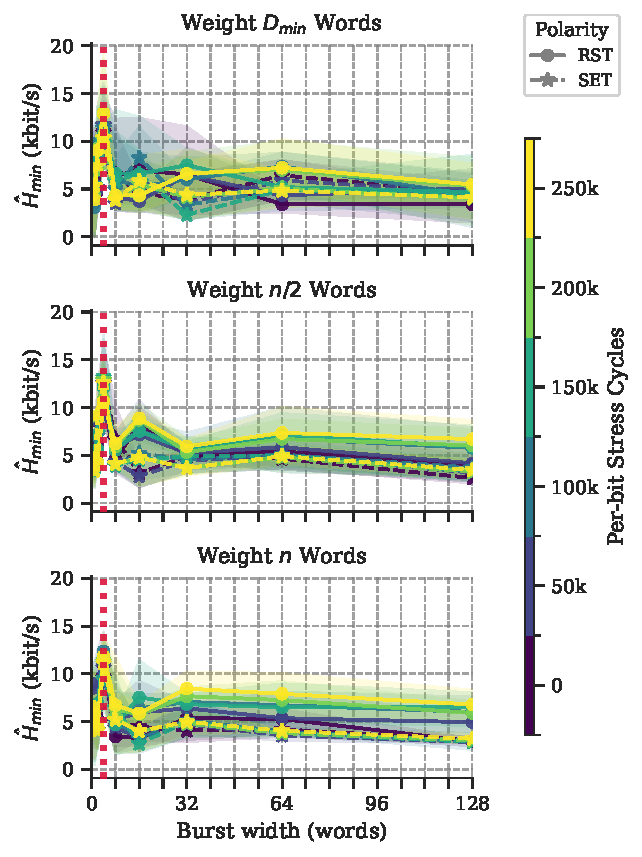
\includegraphics[width=0.5\linewidth]{img/0b_hrate_vs_bw_4m.pdf}
	\vspace{-0.6cm}
	\caption{
		The entropy rate measured over various wear-leveled codeword sequence compositions and burst sizes in an MB85AS4MT 4Mb module from Ramxeed under varying stress levels.
		Each codeword composition is defined by the number of active transitioning bits.
		Several passes are conducted with a uniform stress sequence conducted after each measurement period.
		Clear peaks in entropy efficiency are distinguishable at burst length 4.
		\label{fig:opt-burst4m}
	}
\end{figure}

\subsection{Optimizing Bursted-Write Operations}

\label{sec:opt-burst}
The authors of \cite{sheaves2026brewrc} reverse engineer the physical crossbar dataword size ($k$) from the serialization of write operations with no switching activity. That is, burst operations sequence word-sized write operations. However, burst operations are sequenced far more efficiently than individual, single-word writes.

The all 0's codeword ($\mathbf{0}$) is valid in any linear ECC (i.e. the code forms a vector subspace). That is, a transition is possible from the ($\mathbf{0}$) codeword to any other valid codeword. This property makes it simple to construct codewords of unipolar transitions, which isolate the SET and RESET switching dynamics. By definition, a transition from the all 0's codeword to any other codeword is logically unipolar, biasing the ReRAM in one voltage polarity. A transition back to the all 0's codeword is unipolar in the opposing voltage polarity. 

Without ECC knowledge, the only guaranteed method to obtain latency measurements with identical switching characteristics within a single word is to select a random dataword $u$ producing an unknown codeword $c_?$, and write the sequence $S_? = c_? \rightarrow \mathbf{0} \rightarrow c_?$, where each transition ($\rightarrow$) produces a unipolar latency measurement. This approach asymmetrically wears the bitcells transitioning in $S_?$. Another approach is to write the sequence to many words in a round-robbin fashion. While wear within each word is still asymmetric, the switching duty cycle of each bitcell is significantly reduced.

Given knowledge of the ECC, wear-leveled patterns which include all bits within the word can be constructed. These patterns can be sequenced breadth-first among multiple contiguous words and committed to the memory in a burst. As bursts serialize, many entropic events aggregate and pool yielding cumulative min-entropy gain \cite{nist90b}. We now optimize this bursted test pattern regime. 

As observed in Section \ref{sec:remove-structural} uniform switching eliminates the majority of the structural latency component, leaving a noisy residual. However, uniform swiching can be performed across many bits in order to prevent CF degradation.
We construct three codeword families: \emph{dmin}, \emph{half-weight}, and \emph{full-turnover}, composed entirely of fixed-weight transitions, while keeping per-bit switching counts uniform across each sequence. 

\input{figs/optimal_burst_seq_8m}

\textbf{Minimum-distance sequence.}
Given an $[n,k,d_{\min}]$ linear code with generator matrix $\mathbf{G}$, let $\mathcal{C}$ denote the set of all minimum-weight codewords,
\begin{equation}
    \mathcal{C} = \bigl\{\,\mathbf{u}\mathbf{G} \bmod 2
                  : \mathrm{wt}(\mathbf{u}\mathbf{G}) = d_{\min}\bigr\}.
\end{equation}
Because $|\mathcal{C}|$ is small in both , it is enumerated exhaustively using a simple SAT construction\@. Let $t_j$ be the cumulative toggle count at bit position $j$ when codeword $i$ is used $x_i \geq 0$ times across $L$ total writes. An ILP assigns each codeword a repetition count,
\begin{equation}
\begin{multlined}
    \mathbf{x}^{*} = \arg\min_{\mathbf{x}}\;
                     \Bigl(\max_{j}\,t_j - \min_{j}\,t_j\Bigr)  \\
    \quad \text{subject to} \quad
    \textstyle\sum_{i} x_i = L, \quad x_i \in \mathbb{Z}_{\geq 0},
    \label{eq:ilp}
\end{multlined}
\end{equation}
yielding a provably wear-leveled sequence $\mathcal{S}_{d_{\min}}$. The shortest balanced subset is extracted as $\mathcal{S}_{\mathrm{meas}} \subseteq \mathcal{S}_{d_{\min}}$ for use in timing experiments. For the 4M (8M) module, our solver produces a wear-leveled sequence of 49 (88) $D_{min}$ write operations incurring 7 (10) total transitions per word. For our extracted ECC, this is the optimal solution perfectly satisfying
\begin{equation}
\label{eqn:rt}
    r_t = \frac{n}{r}
\end{equation}
where $r_t < 1$ is the ratio of the number of toggles incurred per write operation over the entire sequence.

% alg2.tex
\begin{algorithm}[t]
\footnotesize
\DontPrintSemicolon
\caption{Wear-leveled burst measurement\label{alg:burst}}
\KwIn{Addresses $\mathcal{A}$, sequences $\mathcal{S}$, widths $\mathcal{W}$, rest fill $f$, rounds $R$}
Write $f$ to all of $\mathcal{A}$\tcp*{initialise}
\For{$\mathrm{round} \leftarrow 1$ \KwTo $R$}{
    \For{$j \leftarrow 0$ \KwTo $N_{\mathrm{buf}}-1$}{
        \ForEach{$a \in \mathcal{A}$, $\mathbf{c} \in \mathcal{S}$, $w \in \mathcal{W}$}{
            Timed write: slots $j$ to $j{+}w{-}1$ get $\mathbf{c}$, remainder get $f$\;
            Write $f$ to $a$\tcp*{restore}
        }
    }
    \If{$\mathrm{round} < R$}{
        Write $\bar{f}$ then $f$ to all of $\mathcal{A}$, $N_{\sigma}$ times
    }
}
\end{algorithm}


\textbf{Half-weight sequence.}
For codewords with $\mathrm{wt} \in \{\lfloor n/2 \rfloor, \lceil n/2 \rceil\}$, exhaustive enumeration is intractable. A pool of $P \gg L$ valid codewords are generated via SAT construction, codewords are then appended greedily, each step selecting the pool candidate that most reduces the running spread $\max_j t_j - \min_j t_j$. This achieves wear-leveling without solving~\eqref{eq:ilp}. Our greedy solver produces the optimal wear-leveled sequence. We do not report the solution here as doing so would reveal $n$ and therefore the ECC strength of the chips.

\textbf{Full-turnover sequence.}
A single all-toggle word of weight $n$ may be simply repeated $|\mathcal{S}_{\mathrm{meas}}|$ times, toggling every bit position on every write. No solver is needed for this sequence as it is trivial to test the existence of the all 1's codeword $\mathbf{1}$ in any linear block code.

\subsection{Bursted Wear-leveled Measurement Sequences}
\label{sec:burst}

An experiment is now performed to demonstrate how bursting and wear-leveled sequences can be combined to form bursted wear-leveled sequences that that maximize the rate at which entropy can be harvested.  

A burst of width $w$ writes $w$ consecutive codeword-sized words in a single 256\,B SPI transaction. By varying $w$ over $[1, N_{\mathrm{buf}}]$, we characterize how entropy scales with burst size. A rotating wear-leveling offset distributes stress evenly across words. Algorithm~\ref{alg:burst} describes bursted wear-leveled measurement sequence generation. After applying the entire sequence to each address, we wear the address using repeated full-turnover bursts across the entire buffer. We repeat this measure-stress-measure routine 7 times. We introduce an entropy efficiency per burst as a performance metric:
\begin{equation}
\dot{H}_{\min}(w) = \hat{H}_{\min}(w)/\bar{\tau}_w
\end{equation}
where $\hat{H}_{\min}(w)$ denotes the estimated min-entropy per measurement (bits) for burst width $w$, computed via NIST SP 800-90B characterization, and $\bar{\tau}_w$ is the mean write latency (cycles) per codeword within the burst. We use this as a coarse grained measurement to estimate the entropy for each operating point explored in the experiment.

Figures \ref{fig:opt-burst4m} and \ref{fig:opt-burst8m} show the results of this experiment on the 4M and 8M modules, respectively. Each write operation in the bursted wear-leveled sequences are applied as entire 256-byte bursted write operations. We apply the entire sequence to 10 256B-aligned addresses, and capture the entropy for each burst-length and wear-leveled write sequence and display the range of $\dot{H}_{\min}(w)$ as ribbons. Across both chips, the results show clear peaks where $\dot{H}_{\min}(w)$ is maximized. Both chips also exhibit higher RESET $\dot{H}_{\min}(w)$ than SET $\dot{H}_{\min}(w)$.
In the next section we implement our entropy source using the highest average $\dot{H}_{\min}(w)$ sequence over the validated wear levels shown in Figures \ref{fig:opt-burst4m} and \ref{fig:opt-burst8m}. For the 4M (8M) the highest average efficiency occurs with 4-word (32-word) bursts consisting of $D_{min}$-weight codeword transitions achieving 15 kbits/sec (40.54 kbit/s).